% !TeX spellcheck = de_DE
\documentclass{alex_gp}
\usepackage[export]{adjustbox}

\name{Alexander Helbok}
\course{Grundpraktikum}
\hwnumber{6}
\spacing{}


\begin{document}
\renewcommand{\labelenumi}{\alph{enumi})}


\begin{mybox}{Stärke und Inklination des Erdmagnetfeldes}
	Ziel dieses Versuches ist es, sowohl den Betrag, als auch die Ausrichtung des Erdmagnetfeldes in Innsbruck zu bestimmen. Dafür wird der Magnetsensor  des IOLab verwendet. Diese muss zuerst kalibriert werden. 
	
	Der Magnetsensor misst das Magnetfeld ich die drei (kartesischen) Raumrichtungen. Um die Berechnung des Magnitude und Inklination des Magnetfeldes zu vereinfachen, drehen wir unser Koordinatensystem (das IOLab) so, dass der Sensor im Rahmen der Unsicherheit einen Wert von 0 in eine Raumrichtung ausgibt. In unserem Fall war das die y-Komponente, welche minimiert wurde. Dann ergibt sich nämlich für den Gesamtbetrag des Erdmagnetfeldes 
	\begin{equation}\label{eqn:mag1}
		|\vec{B}| = \sqrt{B_x^2 + B_z^2}
	\end{equation}
	und für den Inklinationswinkel
	\begin{equation}\label{eqn:theta1}
		\theta = \arctan(\tfrac{B_z}{B_x})
	\end{equation}
	
	Die Messung wurde am Boden durchgeführt durchgeführt und lief etwas über \( 30 \unit{s} \). Die gewonnen Daten sind in \autoref{fig:Bmean} dargestellt. Es wurde für jede Komponente der Mittelwert gebildet und der Fehler auf die Standardabweichung gesetzt, da dann (per Definition) zwei drittel der Daten innerhalb des \( 1\sigma \) Intervalls liegen. 
	
	\begin{figure}[H]	
		\centering
		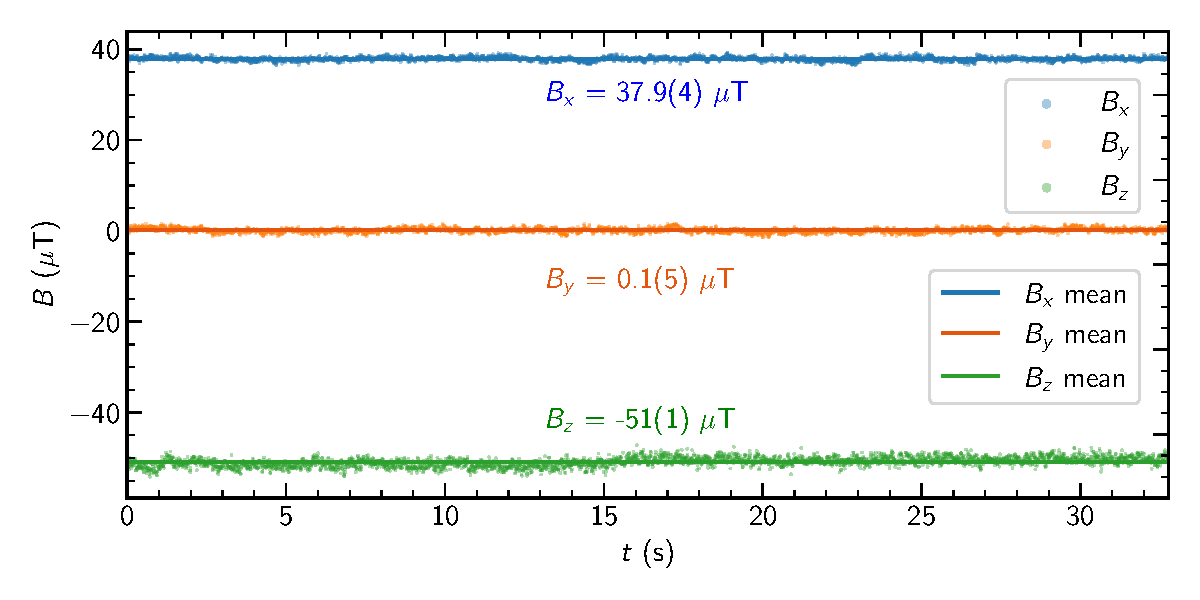
\includegraphics[width=\textwidth]{Versuch6_1}
		\caption{Das gemessene Magnetfeld in die drei kartesischen Raumrichtungen farblich unterscheidbar auf die Zeit aufgetragen. Der Mittelwert der Daten wird als durchgezogene Linie dargestellt.}
		\label{fig:Bmean}
	\end{figure}
	
	Man erhält für die drei kartesischen Komponenten des Erdmagnetfeldes
	\begin{equation}\label{eqn:Bxyz}
		B_x = 37.9(4) \unit{\micro T} \qquad B_y = 0.1(5) \unit{\micro T} \qquad B_z = -50.9(1.0) \unit{\micro T}
	\end{equation}

	Daraus lässt sich jetzt mit \autoref{eqn:mag1} und \autoref{eqn:theta1} die Stärke und Inklination des Erdmagnetfeldes berechnen und man erhält folgende Werte
	\begin{equation}\label{eqn:results}
		|\vec{B}| = 63.4(9) \unit{\micro T} \hspace{3cm} \theta = \ang{53.3(6)}
	\end{equation}
	
	Vergleicht man diese Werte mit Literaturwerten \footnotemark[1]
	\begin{equation}\label{key}
		|\vec{B}| = 48.40(15) \unit{\micro T} \hspace{3cm} \theta = \ang{63.5(2)}
	\end{equation}
	erkennt man, dass unsere gemessenen Werte signifikant abweichen. Das liegt wahrscheinlich daran, dass am Versuchsort eine Vielzahl an metallische Objekte vorhanden waren, die Magnetfelder beeinflussen oder sogar selber erzeugen. Der Versuch wurde nämlich in einem Gebäude aus Stahlbeton durchgeführt, in einem Raum voller Elektronik und oberhalb Labore, in welchen Experimente mit elektrischen und Magnetische Felder durchgeführt werden. Es kommt daher zu systematischen Abweichungen, die verringert werden können, indem man die Messung fern von metallischen Objekten wiederholt.

	\footnotetext[1]{https://www.ngdc.noaa.gov/geomag/calculators/magcalc.shtml\#igrfwmm}
\end{mybox}

\begin{mybox}{Elektromotor}
	In diesem Versuch wird mithilfe der Lorentz Kraft die Polung eines Permanentmagneten bestimmen. Der Versuchsaufbau sah wie folgt aus: Auf den Magneten wurde eine leitende Schraube gestellt, dessen Spitze als Drehachse fungiert. Auf die Schraubenspitze balancieren wir eine Batterie. Das andere Ende der Batterie verbinden wir mit einem Kabel mit dem Magneten. Hierbei ist wichtig, das Kabel am äußeren Rand des Magneten anzuschließen, da es sonst zu keiner Rotation der Batterie kommt.
	
	Die Lorentz Kraft ist so definiert 
	\begin{equation}\label{eqn:Fl}
		\vec{F} = q \vec{v} \times \vec{B}
	\end{equation}
	mit der Ladung \( q \), der Geschwindigkeit der Ladungen \( \vec{v} \) und dem Magnetfeld \( \vec{B} \). Das Magnetfeld in einem Permanentmagneten verläuft annähernd geradlinig vom Südpol zum Nordpol. Das Kreuzprodukt wird maximal, wenn die beiden Vektoren normal aufeinander stehen, also wenn der Strom seitlich in (oder aus) den Magneten fließt, weshalb das Kabel auch an der Seite angebracht wurde. 
	
	Je nach Ausrichtung des Magneten geht das Magnetfeld in die positive oder negative z-Richtung und je nach Ausrichtung der Batterie fließt der Strom von der Batterie über das Kabel in den Magneten oder umgekehrt. Wir haben also vier verschiedene Konfigurationsmöglichkeiten mit zwei unterschiedliche Beobachtungen, eine Drehung in und gegen den Uhrzeigersinn. In \autoref{fig:Motor} ist der Versuchsaufbau (links), sowie die möglichen Konfigurationsarten (rechts) dargestellt.
	
	\begin{figure}[H]
		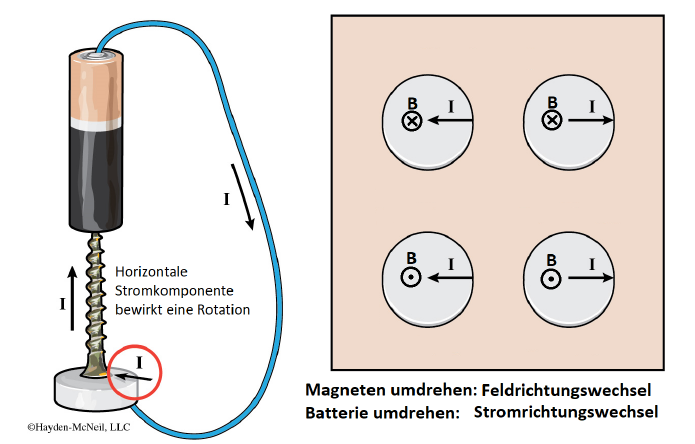
\includegraphics[width=.7\textwidth, right]{Motor}
		\caption[]{Links: Versuchsaufbau des Batteriemotors. Auf einen Permanentmagneten wird über eine Schraube eine Batterie gestellt, welche über ein Kabel wieder mit dem Magneten in der Basis verbunden ist. Rechts: möglichen Konfigurationsarten des Versuchs mit eingezeichnetem Strom und Magnetfeld. Graphik entnommen aus \footnotemark[2] }
		\label{fig:Motor}
	\end{figure}

	\begin{minipage}{\textwidth}
		\vspace{-13cm}
		\begin{tikzpicture}[scale=3]
			\draw[-Stealth] (0,0) -- (0,1) node [above] {\large \( z \)};
			\draw[-Stealth] (0,0) -- (1,0) node [right] {\large \( x \)};
			\draw[-Stealth] (0,0) -- (0.6,0.4) node [right] {\large \( y \)};
			
			\node at (3.2,1.8) {\large \( 1 \)};
			\node at (4,1.8) {\large \( 2 \)};
			\node at (3.2,0.9) {\large \( 3 \)};
			\node at (4,0.9) {\large \( 4 \)};
		\end{tikzpicture}
	\end{minipage}
	
	\begin{center}
		\captionof{table}{Stromrichtung, Drehrichtung und daraus erschlossene Magnetfeldrichtung für die vier Konfigurationen.}
		\begin{tabular}{@{\extracolsep{5mm}} 
				r
				c
				c
				c
			}
			\toprule
			\makecell[t]{Konfiguration}
			&   {\makecell[t]{Stromrichtung}}
			&   {\makecell[t]{Drehrichtung}}
			&   {\makecell[t]{Magnetfeldrichtung}}\\
			\midrule
			1 & \( -\hat{x} \) & \( \circlearrowright \) & \( -\hat{z} \) \\
			2 & \( \hat{x} \) & \( \circlearrowleft \) & \( -\hat{z} \) \\
			3 & \( -\hat{x} \) & \( \circlearrowleft \) & \( \hat{z} \) \\
			4 & \( \hat{x} \) & \( \circlearrowright \) & \( \hat{z} \) \\
			\bottomrule
		\end{tabular}
		\label{table:1}
	\end{center}
	\footnotetext[2]{Angabe}
\end{mybox}

\begin{mybox}{Strom durch Leiter}

\end{mybox}


\end{document}